\section{Overview of Our Approach}
As depicted in Figure~\ref{fig:Figure 4}, the system is proposed as a software protection system within which an obfuscation engine and solving the conflict problem. It mainly obtain three part.

At the first part, we are mainly introduce to how to obfuscate the smali code. The basic idea is confusing the data-flow for the access procedure of register data, and combining opaque predicates technology to confuse the control-flow.

The next step, because our obfuscation method would cause problems of the register-type conflict, we should make the executable .dex file normally execute by the Dalvik VM. So we need to modify the .dex file ,which is  explained in Section 4.3.

Lastly, we will utilize the dex dynamic loading technology to load the above .dex file, but some bytecode is nop after the class being loaded, so Dalvik runtime tampering technology is used to solve the problem. Meanwhile, To illustrate this, we firstly analyzed the exact nature of the problem, and then describe the details process that is to implement normal running.


\begin{figure}[!tbp]
  \centering
  % Requires \usepackage{graphicx}
  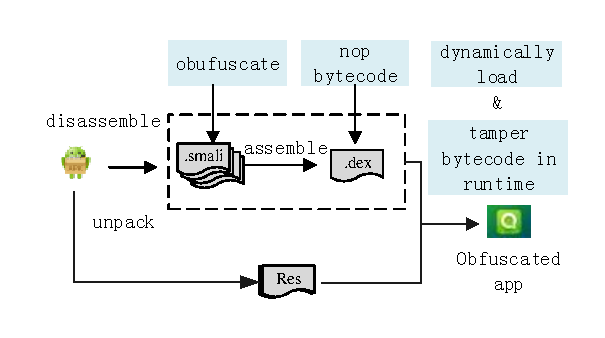
\includegraphics[width=1\columnwidth]{fig/fig4.pdf}
  \caption{Workflow of the SmaliPro system. we can see three part, obfuscate the smali code ,nop bytecode within the .dex file, and dynamic load and runtime tamper, which is the background of the light-green.}\label{fig:Figure 4}
\end{figure}


\section{Implementation details}
In this section, we describe some implementation details for the obfuscation techniques, starting with obfuscating engineering of our approach.
\subsection{Obfuscate the value of register}
Dalvik VM's instructions based on the architecture of register and the constant pool is modified to use the index of 32 bits, which can simplify the interpreter. Therefore the constants within smali code  are stored in the 32-bit registers. According to this characteristic we can confuse the access procedure of constants and control flow, that is data flow obfuscation and control flow obfuscation.

Dalvik VM get the operand from the corresponding register directly based on the type of operation code when perform bytecode flow, regardless of what the type of register is, so we can obfuscate from two aspects. On the one hand, because the constants of the long  and double in smali code are 64-bit, they are stored in the two adjacent 32-bit registers, so we can use a long constant instead of the two constants respectively stored in two 32-bit registers . On the other hand, we will confuse a instruction of capturing the return value of an object reference for a instruction of capturing the return value. The two methods on the above is to confuse on the data access, so that it can make the compiler tools puzzled.

Confusing the control flow is an effective way. its principle is to hide or modify the real control process that adopt various technical, which is to adjust the program structure and the execution path, or to add the opaque predicates and so on to increase the difficulty of the compiler, so that it can prevent the attacker to analysis the control flow of the program\cite{12}.

In this paper, we propose a obfuscation method by inserting reinforced opaque predicates\cite{07}. The first step is to judge the position where to insert, which was conducted on the basis of process analysis. Invoking the key function(\emph{self-define}) is very important modules of program, so we can insert the location of reinforced opaque predicates where is between the instruction of invoking the key function and  the accessing returned value, and the process is shown in Figure~\ref{fig:Figure 5}. For example, the function of purchasing equipment function is very critical in the game and its returned value is usually analyzed by the attacker. If the developer take such protection method, the attackers can't get the return value. This way not only increase the complexity of control flow, but data flow.

\begin{figure}[!tbp]
  \centering
  % Requires \usepackage{graphicx}
  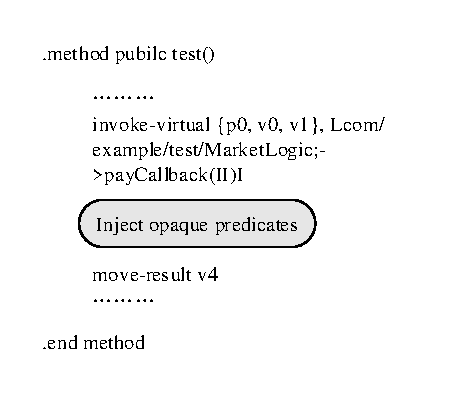
\includegraphics[width=0.8\columnwidth]{fig/fig5.pdf}
  \caption{Control obfuscation. In order to obfuscate the control-flow, we will inject the opaque predicates between two instructions that are invoking and capturing the return value.}\label{fig:Figure 5}
\end{figure}
\subsection{Register type-conflict problem}
Let us consider a small Obfuscated smali method, which is the method of adding two numbers.

\begin{lstlisting}[language={[ANSI]C}, backgroundcolor=\color{backcolour},keywordstyle=\color{blue},commentstyle=\color{red!50!green!50!blue!50}]
.method public static add()I
    const-wide v0, 0x0000000300000002
    add-int v2 , v0,v1
    return v2
.end method

\end{lstlisting}

\noindent The long variable is stored in v0 and v1. When they are to be added, the Dalvik VM will terminate the app and output the following type-conflict error messages to logcat:
\begin{lstlisting}[language={[ANSI]C}, backgroundcolor=\color{backcolour},keywordstyle=\color{blue}]
VEY: register1 v0 type 19, wanted 17
VEY: register1 v1 type 20, wanted 17
VEY: rejecting opcode 0x90 at 0x0008
VEY: rejected Lcom/example/****/****;
.add()I
Verifier rejected class Lcom/example/
****/****;
Class init failed in newInstance

\end{lstlisting}

We can see this register-type conflict problem from the static program analysis'viewpoint follows. The verifier module\cite{35,36} to perform a register type analysis each method within a class prior to running it, and ensure that there is no type conflict. Should it the register with two diffirent types at the same method when loading the class, it will then report the register-type conflict problem as shown above.

Given this issue, we thus need to find a solution that will bypass the verifier of the evaluated Android runtime systems from deducing any false type conflict in otherwise correctly obfuscated apps.




\subsection{App execution}
As shown in Figure~\ref{fig:Figure 3}, Dalvik VM verifies the validity of instructions when loading the class, for example, verifying the type of the registers. so executing an obfuscated app must bypass the process of the verifier.To address the problem, we can do the following three things.

\begin{enumerate}[leftmargin=*]
\item[(i)] First of all, we will recompile the obfuscated smali into a .dex file . Then the bytecode of each obfuscated method which is in the .dex file can be stored in the ObjMethod structure of showing in Figure~\ref{fig:Figure 6}. At last, we will fill the zero bytecode in the obfuscated method and get a new.dex file. This way resist static analysis successfully.

\item[(ii)] In order to load the executable file new.dex utilizing the technology of loading dex dynamically, we develop our own customized Classloader to load all the classes in this dex file, before which the default Classloader in the API layer should be replaced to ensure the normal execution of the real dex file.

    There exists a system component called Application[14] in Android frame. it will initialize several global variables when establishing Application(i.e. before launching app ),  and all the Activity within the same app can access the value of these variables. Usually, system will develop an Application automatically and we don't need to develop it specifically, so through designing customized class ProxyApplication that extends  Application, the default Classloader in the system will be replaced by the customized MyDexclassloder when initiating ProxyApplication. Moreover, we should configure ProxyApplication in the ApplicationManifest.xml file as folllows:
    \begin{lstlisting}[language={[ANSI]C}, backgroundcolor=\color{backcolour},keywordstyle=\color{blue!70},commentstyle=\color{red!50!green!50!blue!50}]
    <application
      Android:name="ProxyApplication"
    </application
    \end{lstlisting}


\item[(iii)] In order to bypass verification of Dalvik VM for instructions(i.e. register types), we utilize  the technology of dynamically loading. As bytecode in the obfuscated  methods  in new.dex is a zero sequence after loading new.dex, we need to fill the obfuscated bytecode in the corresponding location in the memory before execution.

    \par When running an Android appication, it will load dex file and parse the dalvik bytecode that is executed by Dalvik VM. We reads or writs the byte flow when running the app with the aid of the JNI component\cite{15}, as there isn't a direct method to achieve this compared to X86 and ARM frame due to limited instruction sets of DVM. Native library and Dalvik VM owe the same priority as they are in the same process, so we can utilize JNI to call methods in native library to achieve the modification for Dalvik bytecode.

    The address of dex in the memory after loading can be acquired through DexFile class in Android system. According to the address, we can acquire the memory address of the obfuscated methods via parsing the dex structure, then fill in the corresponding memory address with the corresponding  bytecode stored in the ObjMethod structure to ensure correct system execution.
\end{enumerate}

\begin{figure}[!tbp]
  \centering
  % Requires \usepackage{graphicx}
  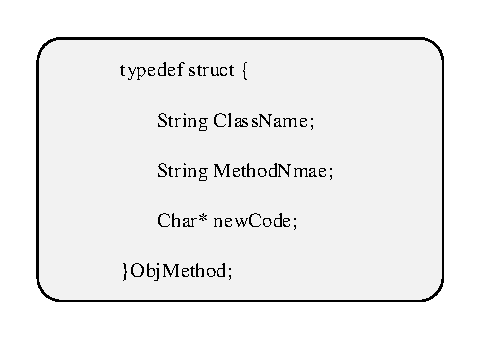
\includegraphics[width=0.8\columnwidth]{fig/fig6.pdf}
  \caption{The structure of ObjMethod. It is used to store the bytecode of the obfuscated method within the .dex file. The bytecode backfill the memory after the class loaded}\label{fig:Figure 6}
\end{figure}